% Created by tikzDevice version 0.12.3 on 2019-12-11 20:53:31
% !TEX encoding = UTF-8 Unicode
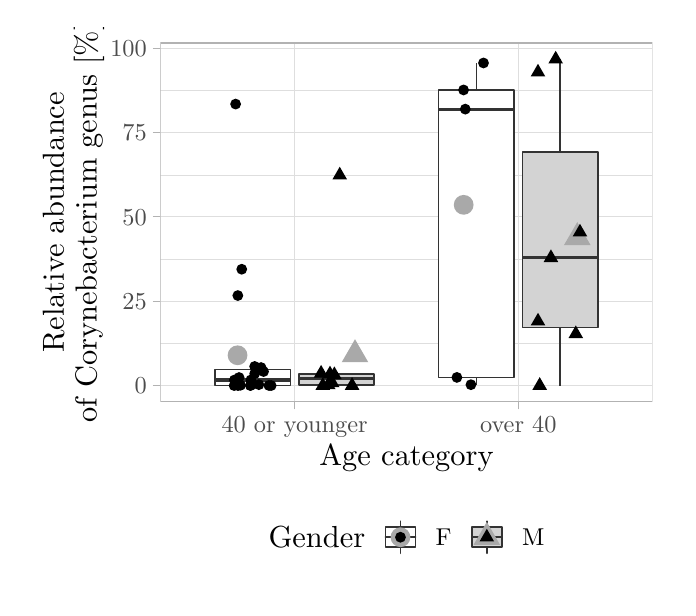
\begin{tikzpicture}[x=1pt,y=1pt]
\definecolor{fillColor}{RGB}{255,255,255}
\path[use as bounding box,fill=fillColor,fill opacity=0.00] (0,0) rectangle (231.26,202.36);
\begin{scope}
\path[clip] (  0.00,  0.00) rectangle (231.26,202.36);
\definecolor{drawColor}{RGB}{255,255,255}
\definecolor{fillColor}{RGB}{255,255,255}

\path[draw=drawColor,line width= 0.6pt,line join=round,line cap=round,fill=fillColor] (  0.00,  0.00) rectangle (231.26,202.36);
\end{scope}
\begin{scope}
\path[clip] ( 47.99, 67.14) rectangle (225.76,196.86);
\definecolor{fillColor}{RGB}{255,255,255}

\path[fill=fillColor] ( 47.99, 67.14) rectangle (225.76,196.86);
\definecolor{drawColor}{gray}{0.87}

\path[draw=drawColor,line width= 0.1pt,line join=round] ( 47.99, 88.28) --
	(225.76, 88.28);

\path[draw=drawColor,line width= 0.1pt,line join=round] ( 47.99,118.75) --
	(225.76,118.75);

\path[draw=drawColor,line width= 0.1pt,line join=round] ( 47.99,149.23) --
	(225.76,149.23);

\path[draw=drawColor,line width= 0.1pt,line join=round] ( 47.99,179.71) --
	(225.76,179.71);

\path[draw=drawColor,line width= 0.3pt,line join=round] ( 47.99, 73.04) --
	(225.76, 73.04);

\path[draw=drawColor,line width= 0.3pt,line join=round] ( 47.99,103.52) --
	(225.76,103.52);

\path[draw=drawColor,line width= 0.3pt,line join=round] ( 47.99,133.99) --
	(225.76,133.99);

\path[draw=drawColor,line width= 0.3pt,line join=round] ( 47.99,164.47) --
	(225.76,164.47);

\path[draw=drawColor,line width= 0.3pt,line join=round] ( 47.99,194.95) --
	(225.76,194.95);

\path[draw=drawColor,line width= 0.3pt,line join=round] ( 96.47, 67.14) --
	( 96.47,196.86);

\path[draw=drawColor,line width= 0.3pt,line join=round] (177.28, 67.14) --
	(177.28,196.86);

\path[] ( 81.32,115.07) circle (  1.96);

\path[] ( 81.32,105.56) circle (  1.96);

\path[] ( 81.32,174.75) circle (  1.96);
\definecolor{drawColor}{gray}{0.20}

\path[draw=drawColor,line width= 0.6pt,line join=round] ( 81.32, 78.82) -- ( 81.32, 79.94);

\path[draw=drawColor,line width= 0.6pt,line join=round] ( 81.32, 73.11) -- ( 81.32, 73.04);

\path[draw=drawColor,line width= 0.6pt,line join=round,line cap=round,fill=fillColor] ( 67.69, 78.82) --
	( 67.69, 73.11) --
	( 94.96, 73.11) --
	( 94.96, 78.82) --
	( 67.69, 78.82) --
	cycle;

\path[draw=drawColor,line width= 1.1pt,line join=round] ( 67.69, 75.04) -- ( 94.96, 75.04);

\path[] (111.63,149.06) circle (  1.96);

\path[draw=drawColor,line width= 0.6pt,line join=round] (111.63, 77.24) -- (111.63, 77.44);

\path[draw=drawColor,line width= 0.6pt,line join=round] (111.63, 73.21) -- (111.63, 73.04);
\definecolor{fillColor}{RGB}{211,211,211}

\path[draw=drawColor,line width= 0.6pt,line join=round,line cap=round,fill=fillColor] ( 97.99, 77.24) --
	( 97.99, 73.21) --
	(125.26, 73.21) --
	(125.26, 77.24) --
	( 97.99, 77.24) --
	cycle;

\path[draw=drawColor,line width= 1.1pt,line join=round] ( 97.99, 75.44) -- (125.26, 75.44);

\path[draw=drawColor,line width= 0.6pt,line join=round] (162.13,179.85) -- (162.13,189.60);

\path[draw=drawColor,line width= 0.6pt,line join=round] (162.13, 75.98) -- (162.13, 73.35);
\definecolor{fillColor}{RGB}{255,255,255}

\path[draw=drawColor,line width= 0.6pt,line join=round,line cap=round,fill=fillColor] (148.49,179.85) --
	(148.49, 75.98) --
	(175.77, 75.98) --
	(175.77,179.85) --
	(148.49,179.85) --
	cycle;

\path[draw=drawColor,line width= 1.1pt,line join=round] (148.49,172.92) -- (175.77,172.92);

\path[draw=drawColor,line width= 0.6pt,line join=round] (192.43,157.34) -- (192.43,190.96);

\path[draw=drawColor,line width= 0.6pt,line join=round] (192.43, 93.99) -- (192.43, 73.04);
\definecolor{fillColor}{RGB}{211,211,211}

\path[draw=drawColor,line width= 0.6pt,line join=round,line cap=round,fill=fillColor] (178.80,157.34) --
	(178.80, 93.99) --
	(206.07, 93.99) --
	(206.07,157.34) --
	(178.80,157.34) --
	cycle;

\path[draw=drawColor,line width= 1.1pt,line join=round] (178.80,119.20) -- (206.07,119.20);
\definecolor{fillColor}{RGB}{169,169,169}

\path[fill=fillColor] (118.28, 89.78) --
	(123.08, 81.46) --
	(113.47, 81.46) --
	cycle;

\path[fill=fillColor] ( 75.84, 83.98) circle (  3.57);

\path[fill=fillColor] (198.60,132.10) --
	(203.41,123.78) --
	(193.79,123.78) --
	cycle;

\path[fill=fillColor] (157.55,138.34) circle (  3.57);
\definecolor{fillColor}{RGB}{0,0,0}

\path[fill=fillColor] (106.64, 76.09) --
	(109.28, 71.51) --
	(104.00, 71.51) --
	cycle;

\path[fill=fillColor] (110.06, 77.01) --
	(112.70, 72.43) --
	(107.42, 72.43) --
	cycle;

\path[fill=fillColor] (106.03, 80.49) --
	(108.68, 75.92) --
	(103.39, 75.92) --
	cycle;

\path[fill=fillColor] (117.22, 76.09) --
	(119.87, 71.51) --
	(114.58, 71.51) --
	cycle;

\path[fill=fillColor] (108.60, 76.31) --
	(111.24, 71.74) --
	(105.95, 71.74) --
	cycle;

\path[fill=fillColor] (112.76,152.11) --
	(115.40,147.53) --
	(110.12,147.53) --
	cycle;

\path[fill=fillColor] (109.24, 80.22) --
	(111.88, 75.64) --
	(106.59, 75.64) --
	cycle;

\path[fill=fillColor] (110.82, 79.97) --
	(113.46, 75.39) --
	(108.17, 75.39) --
	cycle;

\path[fill=fillColor] ( 76.40, 75.94) circle (  1.96);

\path[fill=fillColor] ( 76.01, 73.04) circle (  1.96);

\path[fill=fillColor] ( 84.34, 79.54) circle (  1.96);

\path[fill=fillColor] ( 87.98, 73.04) circle (  1.96);

\path[fill=fillColor] ( 77.35,115.07) circle (  1.96);

\path[fill=fillColor] ( 74.70, 75.04) circle (  1.96);

\path[fill=fillColor] ( 75.94,105.56) circle (  1.96);

\path[fill=fillColor] ( 80.66, 75.07) circle (  1.96);

\path[fill=fillColor] ( 76.92, 73.15) circle (  1.96);

\path[fill=fillColor] ( 85.23, 78.10) circle (  1.96);

\path[fill=fillColor] ( 80.59, 73.15) circle (  1.96);

\path[fill=fillColor] ( 82.02, 79.94) circle (  1.96);

\path[fill=fillColor] ( 87.17, 73.07) circle (  1.96);

\path[fill=fillColor] ( 75.14,174.75) circle (  1.96);

\path[fill=fillColor] ( 80.47, 73.04) circle (  1.96);

\path[fill=fillColor] ( 74.61, 73.04) circle (  1.96);

\path[fill=fillColor] ( 75.44, 74.29) circle (  1.96);

\path[fill=fillColor] ( 82.03, 77.35) circle (  1.96);

\path[fill=fillColor] ( 83.54, 73.37) circle (  1.96);

\path[fill=fillColor] (189.08,122.25) --
	(191.72,117.68) --
	(186.44,117.68) --
	cycle;

\path[fill=fillColor] (185.02, 76.09) --
	(187.66, 71.51) --
	(182.37, 71.51) --
	cycle;

\path[fill=fillColor] (184.40,189.31) --
	(187.04,184.73) --
	(181.76,184.73) --
	cycle;

\path[fill=fillColor] (184.41, 99.33) --
	(187.05, 94.75) --
	(181.76, 94.75) --
	cycle;

\path[fill=fillColor] (198.07, 94.77) --
	(200.71, 90.19) --
	(195.43, 90.19) --
	cycle;

\path[fill=fillColor] (199.57,131.48) --
	(202.22,126.90) --
	(196.93,126.90) --
	cycle;

\path[fill=fillColor] (190.79,194.01) --
	(193.44,189.43) --
	(188.15,189.43) --
	cycle;

\path[fill=fillColor] (164.71,189.60) circle (  1.96);

\path[fill=fillColor] (158.13,172.92) circle (  1.96);

\path[fill=fillColor] (155.10, 75.98) circle (  1.96);

\path[fill=fillColor] (157.51,179.85) circle (  1.96);

\path[fill=fillColor] (160.17, 73.35) circle (  1.96);
\definecolor{drawColor}{gray}{0.70}

\path[draw=drawColor,line width= 0.6pt,line join=round,line cap=round] ( 47.99, 67.14) rectangle (225.76,196.86);
\end{scope}
\begin{scope}
\path[clip] (  0.00,  0.00) rectangle (231.26,202.36);
\definecolor{drawColor}{gray}{0.30}

\node[text=drawColor,anchor=base east,inner sep=0pt, outer sep=0pt, scale=  0.88] at ( 43.04, 70.01) {0};

\node[text=drawColor,anchor=base east,inner sep=0pt, outer sep=0pt, scale=  0.88] at ( 43.04,100.48) {25};

\node[text=drawColor,anchor=base east,inner sep=0pt, outer sep=0pt, scale=  0.88] at ( 43.04,130.96) {50};

\node[text=drawColor,anchor=base east,inner sep=0pt, outer sep=0pt, scale=  0.88] at ( 43.04,161.44) {75};

\node[text=drawColor,anchor=base east,inner sep=0pt, outer sep=0pt, scale=  0.88] at ( 43.04,191.92) {100};
\end{scope}
\begin{scope}
\path[clip] (  0.00,  0.00) rectangle (231.26,202.36);
\definecolor{drawColor}{gray}{0.70}

\path[draw=drawColor,line width= 0.3pt,line join=round] ( 45.24, 73.04) --
	( 47.99, 73.04);

\path[draw=drawColor,line width= 0.3pt,line join=round] ( 45.24,103.52) --
	( 47.99,103.52);

\path[draw=drawColor,line width= 0.3pt,line join=round] ( 45.24,133.99) --
	( 47.99,133.99);

\path[draw=drawColor,line width= 0.3pt,line join=round] ( 45.24,164.47) --
	( 47.99,164.47);

\path[draw=drawColor,line width= 0.3pt,line join=round] ( 45.24,194.95) --
	( 47.99,194.95);
\end{scope}
\begin{scope}
\path[clip] (  0.00,  0.00) rectangle (231.26,202.36);
\definecolor{drawColor}{gray}{0.70}

\path[draw=drawColor,line width= 0.3pt,line join=round] ( 96.47, 64.39) --
	( 96.47, 67.14);

\path[draw=drawColor,line width= 0.3pt,line join=round] (177.28, 64.39) --
	(177.28, 67.14);
\end{scope}
\begin{scope}
\path[clip] (  0.00,  0.00) rectangle (231.26,202.36);
\definecolor{drawColor}{gray}{0.30}

\node[text=drawColor,anchor=base,inner sep=0pt, outer sep=0pt, scale=  0.88] at ( 96.47, 56.13) {40 or younger};

\node[text=drawColor,anchor=base,inner sep=0pt, outer sep=0pt, scale=  0.88] at (177.28, 56.13) {over 40};
\end{scope}
\begin{scope}
\path[clip] (  0.00,  0.00) rectangle (231.26,202.36);
\definecolor{drawColor}{RGB}{0,0,0}

\node[text=drawColor,anchor=base,inner sep=0pt, outer sep=0pt, scale=  1.10] at (136.88, 44.09) {Age category};
\end{scope}
\begin{scope}
\path[clip] (  0.00,  0.00) rectangle (231.26,202.36);
\definecolor{drawColor}{RGB}{0,0,0}

\node[text=drawColor,rotate= 90.00,anchor=base,inner sep=0pt, outer sep=0pt, scale=  1.10] at ( 13.08,132.00) {Relative abundance };

\node[text=drawColor,rotate= 90.00,anchor=base,inner sep=0pt, outer sep=0pt, scale=  1.10] at ( 24.96,132.00) { of Corynebacterium genus [\%]};
\end{scope}
\begin{scope}
\path[clip] (  0.00,  0.00) rectangle (231.26,202.36);
\definecolor{fillColor}{RGB}{255,255,255}

\path[fill=fillColor] ( 81.55,  5.50) rectangle (192.20, 30.95);
\end{scope}
\begin{scope}
\path[clip] (  0.00,  0.00) rectangle (231.26,202.36);
\definecolor{drawColor}{RGB}{0,0,0}

\node[text=drawColor,anchor=base west,inner sep=0pt, outer sep=0pt, scale=  1.10] at ( 87.05, 14.44) {Gender};
\end{scope}
\begin{scope}
\path[clip] (  0.00,  0.00) rectangle (231.26,202.36);
\definecolor{fillColor}{RGB}{255,255,255}

\path[fill=fillColor] (127.49, 11.00) rectangle (141.94, 25.45);
\end{scope}
\begin{scope}
\path[clip] (  0.00,  0.00) rectangle (231.26,202.36);
\definecolor{drawColor}{gray}{0.20}

\path[draw=drawColor,line width= 0.6pt,line join=round,line cap=round] (134.71, 12.45) --
	(134.71, 14.61);

\path[draw=drawColor,line width= 0.6pt,line join=round,line cap=round] (134.71, 21.84) --
	(134.71, 24.01);
\definecolor{fillColor}{RGB}{255,255,255}

\path[draw=drawColor,line width= 0.6pt,line join=round,line cap=round,fill=fillColor] (129.29, 14.61) rectangle (140.13, 21.84);

\path[draw=drawColor,line width= 0.6pt,line join=round,line cap=round] (129.29, 18.23) --
	(140.13, 18.23);
\end{scope}
\begin{scope}
\path[clip] (  0.00,  0.00) rectangle (231.26,202.36);
\definecolor{fillColor}{RGB}{169,169,169}

\path[fill=fillColor] (134.71, 18.23) circle (  3.57);
\end{scope}
\begin{scope}
\path[clip] (  0.00,  0.00) rectangle (231.26,202.36);
\definecolor{fillColor}{RGB}{0,0,0}

\path[fill=fillColor] (134.71, 18.23) circle (  1.96);
\end{scope}
\begin{scope}
\path[clip] (  0.00,  0.00) rectangle (231.26,202.36);
\definecolor{fillColor}{RGB}{255,255,255}

\path[fill=fillColor] (158.68, 11.00) rectangle (173.14, 25.45);
\end{scope}
\begin{scope}
\path[clip] (  0.00,  0.00) rectangle (231.26,202.36);
\definecolor{drawColor}{gray}{0.20}

\path[draw=drawColor,line width= 0.6pt,line join=round,line cap=round] (165.91, 12.45) --
	(165.91, 14.61);

\path[draw=drawColor,line width= 0.6pt,line join=round,line cap=round] (165.91, 21.84) --
	(165.91, 24.01);
\definecolor{fillColor}{RGB}{211,211,211}

\path[draw=drawColor,line width= 0.6pt,line join=round,line cap=round,fill=fillColor] (160.49, 14.61) rectangle (171.33, 21.84);

\path[draw=drawColor,line width= 0.6pt,line join=round,line cap=round] (160.49, 18.23) --
	(171.33, 18.23);
\end{scope}
\begin{scope}
\path[clip] (  0.00,  0.00) rectangle (231.26,202.36);
\definecolor{fillColor}{RGB}{169,169,169}

\path[fill=fillColor] (165.91, 23.78) --
	(170.72, 15.45) --
	(161.10, 15.45) --
	cycle;
\end{scope}
\begin{scope}
\path[clip] (  0.00,  0.00) rectangle (231.26,202.36);
\definecolor{fillColor}{RGB}{0,0,0}

\path[fill=fillColor] (165.91, 21.28) --
	(168.55, 16.70) --
	(163.27, 16.70) --
	cycle;
\end{scope}
\begin{scope}
\path[clip] (  0.00,  0.00) rectangle (231.26,202.36);
\definecolor{drawColor}{RGB}{0,0,0}

\node[text=drawColor,anchor=base west,inner sep=0pt, outer sep=0pt, scale=  0.88] at (147.44, 15.20) {F};
\end{scope}
\begin{scope}
\path[clip] (  0.00,  0.00) rectangle (231.26,202.36);
\definecolor{drawColor}{RGB}{0,0,0}

\node[text=drawColor,anchor=base west,inner sep=0pt, outer sep=0pt, scale=  0.88] at (178.64, 15.20) {M};
\end{scope}
\end{tikzpicture}
